\documentclass[tikz, border=18pt]{standalone}
\usepackage{tikz}
\usepackage{amsmath}
\usepackage{amssymb}
\usetikzlibrary{positioning, arrows.meta, shadows, backgrounds}

% ── Colour palette ────────────────────────────────────────────────────────────
\definecolor{bg}{HTML}{0f1117}          % near-black background
\definecolor{nodebase}{HTML}{1e2235}    % default node fill
\definecolor{infamily}{HTML}{3b5bdb}    % in family, element 1 absent
\definecolor{hasone}{HTML}{e03131}      % in family, contains element 1 (the "winner")
\definecolor{notinfamily}{HTML}{2c2f3f} % not in family
\definecolor{edgecolor}{HTML}{4a5080}
\definecolor{labelcolor}{HTML}{c8d0e8}
\definecolor{titlecolor}{HTML}{ffffff}
\definecolor{subtitlecolor}{HTML}{7c8aad}
\definecolor{highlight}{HTML}{ffd43b}   % element-1 label highlight

\begin{document}
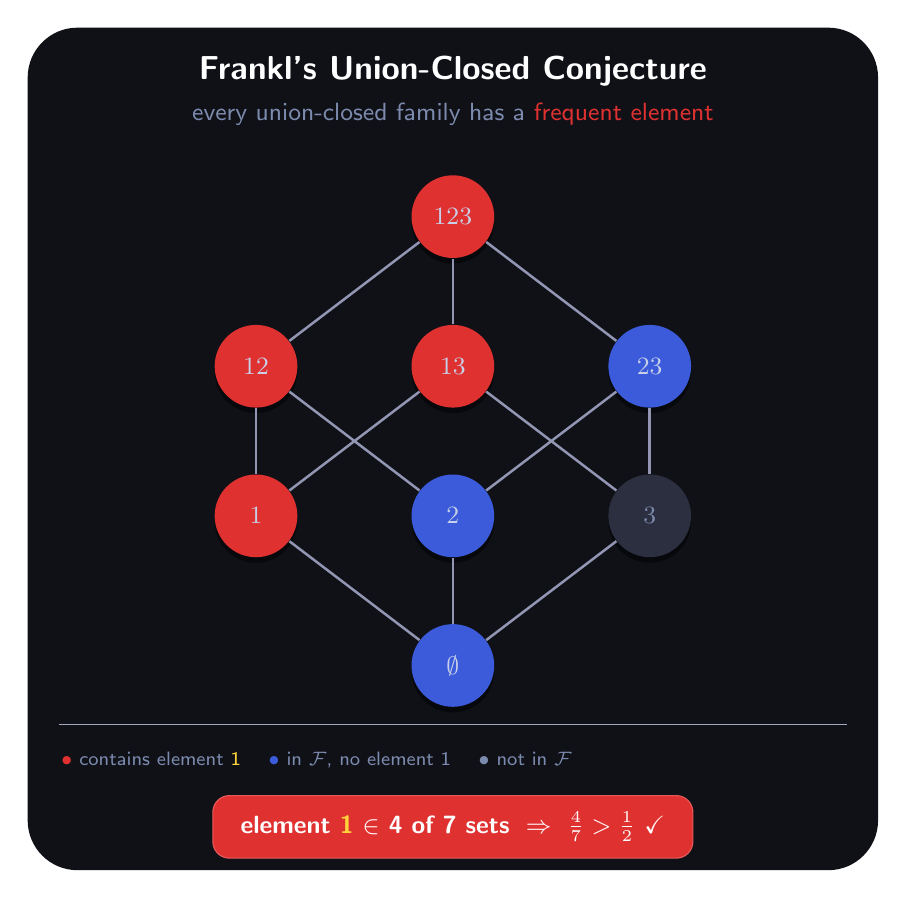
\begin{tikzpicture}[
  % node styles
  set/.style={
    circle, minimum size=1.05cm, inner sep=0pt,
    draw=none, text=labelcolor,
    font=\small\sffamily,
    drop shadow={shadow xshift=0pt, shadow yshift=-2pt,
                 opacity=0.5, fill=black}
  },
  infam/.style={set, fill=infamily},
  hasone/.style={set, fill=hasone},
  notfam/.style={set, fill=notinfamily, text=subtitlecolor},
  % edge style
  hasse/.style={draw=edgecolor, line width=1.2pt, -{Stealth[length=5pt]}},
  hasseplain/.style={draw=edgecolor!60, line width=0.9pt},
]

%% ── Background rectangle ───────────────────────────────────────────────────
\begin{scope}[on background layer]
  \fill[bg, rounded corners=18pt] (-5.4,-3.3) rectangle (5.4,7.4);
\end{scope}

%% ── Title ──────────────────────────────────────────────────────────────────
\node[text=titlecolor, font=\large\bfseries\sffamily] at (0, 6.85)
  {Frankl's Union-Closed Conjecture};
\node[text=subtitlecolor, font=\small\sffamily] at (0, 6.3)
  {every union-closed family has a \textcolor{hasone}{frequent element}};

%% ── Hasse diagram of P([3]) ─────────────────────────────────────────────────
%%    Family F = {∅, {1}, {2}, {1,2}, {1,3}, {2,3}, {1,2,3}}
%%    Element 1 appears in {1},{1,2},{1,3},{1,2,3} = 4 of 7 sets  (> 1/2)
%%    Red  = contains element 1 (the "winner")
%%    Blue = in family, does not contain 1
%%    Dark = not in family

% Level 3 — top
\node[hasone]  (abc) at ( 0.0, 5.0) {$123$};

% Level 2
\node[hasone]  (ab)  at (-2.5, 3.1) {$12$};
\node[hasone]  (ac)  at ( 0.0, 3.1) {$13$};
\node[infam]   (bc)  at ( 2.5, 3.1) {$23$};

% Level 1
\node[hasone]  (a)   at (-2.5, 1.2) {$1$};
\node[infam]   (b)   at ( 0.0, 1.2) {$2$};
\node[notfam]  (c)   at ( 2.5, 1.2) {$3$};

% Level 0 — bottom
\node[infam]   (emp) at ( 0.0,-0.7) {$\emptyset$};

%% edges (upward = union direction)
\foreach \from/\to in {emp/a, emp/b, emp/c,
                        a/ab, a/ac, b/ab, b/bc, c/ac, c/bc,
                        ab/abc, ac/abc, bc/abc}
  \draw[hasseplain] (\from) -- (\to);

%% ── Divider line ─────────────────────────────────────────────────────────────
\draw[edgecolor!50, line width=0.6pt] (-5.0,-1.45) -- (5.0,-1.45);

%% ── Legend ──────────────────────────────────────────────────────────────────
\node[text=subtitlecolor, font=\scriptsize\sffamily, anchor=west] at (-5.1,-1.9)
  {\textcolor{hasone}{$\bullet$} contains element \textcolor{highlight}{1}
   \quad
   \textcolor{infamily}{$\bullet$} in $\mathcal{F}$, no element 1
   \quad
   \textcolor{subtitlecolor}{$\bullet$} not in $\mathcal{F}$};

%% ── Annotation: element-1 fraction ─────────────────────────────────────────
\node[draw=hasone!80, rounded corners=6pt,
      fill=hasone,                        % solid red background
      text=white, font=\small\bfseries\sffamily,
      inner xsep=10pt, inner ysep=6pt] at (0,-2.75)
  {element \textcolor{highlight}{1} $\in$ 4 of 7 sets
   $\;\Rightarrow\;$ $\tfrac{4}{7} > \tfrac{1}{2}$ \checkmark};

%% ── extend background to fit ─────────────────────────────────────────────────
\end{tikzpicture}
\end{document}
